Suppose we have
%\begin{multicols}{2}
\begin{itemize}
	\item binary columns $\bit{1}$, $\bit{2}$, $\bit{3}$, $\bit{4}$, $\bit{5}$
	\item counter constant columns \source{}, \targetOne{}, \targetTwo{}, $\targetOne{}\new{}$, $\targetTwo{}\new{}$
	\item byte columns \source{}\byte{}, \targetOne{}\byte{} and \targetTwo{}\byte{},
	\item counter constant columns \source{}\mark{} and \targetOne{}\mark{},
	\item a counter constant column \size{},
	\item ``accumulator'' columns \acc{1}, \acc{2}, \acc{3}, \acc{4};
	\item a ``power''column \col{P},
	\item a ``counter column'' \ct{}.
		%\item[\vspace{\fill}]
\end{itemize}
%\end{multicols}
The interpretation is as follows: 
\source{}, \targetOne{} and \targetTwo{} are counter-constant columns containing limbs viewed respectively as a ``source'' and two ``target'' limbs; 
\source{}\byte{}, \targetOne{}\byte{} and \targetTwo{}\byte{} are their respective byte decomposition;
$\targetOne{}\new$ and $\targetTwo{}\new$ contain the ``new'' value of \targetOne{} and \targetTwo{} respectively; 
\source{}\mark{} and \target{}\mark{} are markers $\in\{0,1,\dots,\llargeMO\}$ for \source{} and \targetOne{} respectively.
We expect both
$\source{}\mark{} + (\size{}-1)\leq \llargeMO$ and
$\target{}\mark{} + (\size{}-1)\geq \llarge$.
Compare with figure~\ref{fig: one partial to two}.

We collect the following constraints under a collective name: %\ob{TODO}
\begin{enumerate}
	\item plateau constraints
		\begin{enumerate}
			\item $\plateau(\bit{1}, \targetOne{}\mark{}; \ct{})$
			\item $\plateau(\bit{2}, \targetOne{}\mark{} + \size{} - \llarge; \ct{})$
			\item $\plateau(\bit{3}, \source{}\mark{}; \ct{})$
			\item $\plateau(\bit{4}, \source{}\mark{} + \llarge - \targetOne{}\mark{}; \ct{})$
			\item $\plateau(\bit{5}, \source{}\mark{} + \size{}; \ct{})$
		\end{enumerate}
	\item prefix, suffix and chunk constraints:
		\begin{enumerate}
			\item $\compSuffix(\acc{1}, \targetOne{}\byte{}, \bit{1}; \ct{})$, %i.e. $\acc{1}\implies \alpha'$
			\item $\compPrefix(\acc{2}, \targetTwo{}\byte{}, \bit{2}; \ct{})$, %i.e. $\acc{2}\implies \beta$
			\item $\compChunk(\acc{3}, \source{}\byte{}, \bit{3}, \bit{4}; \ct{})$, %i.e. $\acc{3}\implies \gamma$
			\item $\compChunk(\acc{4}, \source{}\byte{}, \bit{4}, \bit{5}; \ct{})$, %i.e. $\acc{4}\implies \gamma'$
		\end{enumerate}
	\item power-constraint: $\power(\col{P},\bit{2}; \ct{})$
	\item update constraint:
		\[
			\If
			\ct_i = \llargeMO~
			\Then
			\begin{cases}
				\targetOne{}\new{}_i
				=
				\targetOne{}_i
				+
				(\acc{3}_i - \acc{1}_i)\\
				\targetTwo{}\new{}_i
				=
				\targetTwo{}_i
				+
				(\acc{4}_i - \acc{2}_i)\cdot\col{P}_i.
			\end{cases}
		\]
\end{enumerate}
We encapsulate all these constraints under a single relation
\[
	\onePartialToTwo
	\left( \begin{array}{c}
		\source{}, \targetOne{}, \targetTwo{},
		\targetOne{}\new, \targetTwo{}\new;
		\source{}\byte{}, \targetOne{}\byte{}, \targetTwo{}\byte{};
		\\
		\acc{1}, \acc{2}, \acc{3}, \acc{4}; \col{P};
		\\
		\source{}\mark{}, \targetOne{}\mark{}, \size{};
		\\
		\bit{1}, \bit{2}, \bit{3}, \bit{4}, \bit{5}; \ct{};
	\end{array} \right)
\]

\begin{figure}[h!]
	\centering
	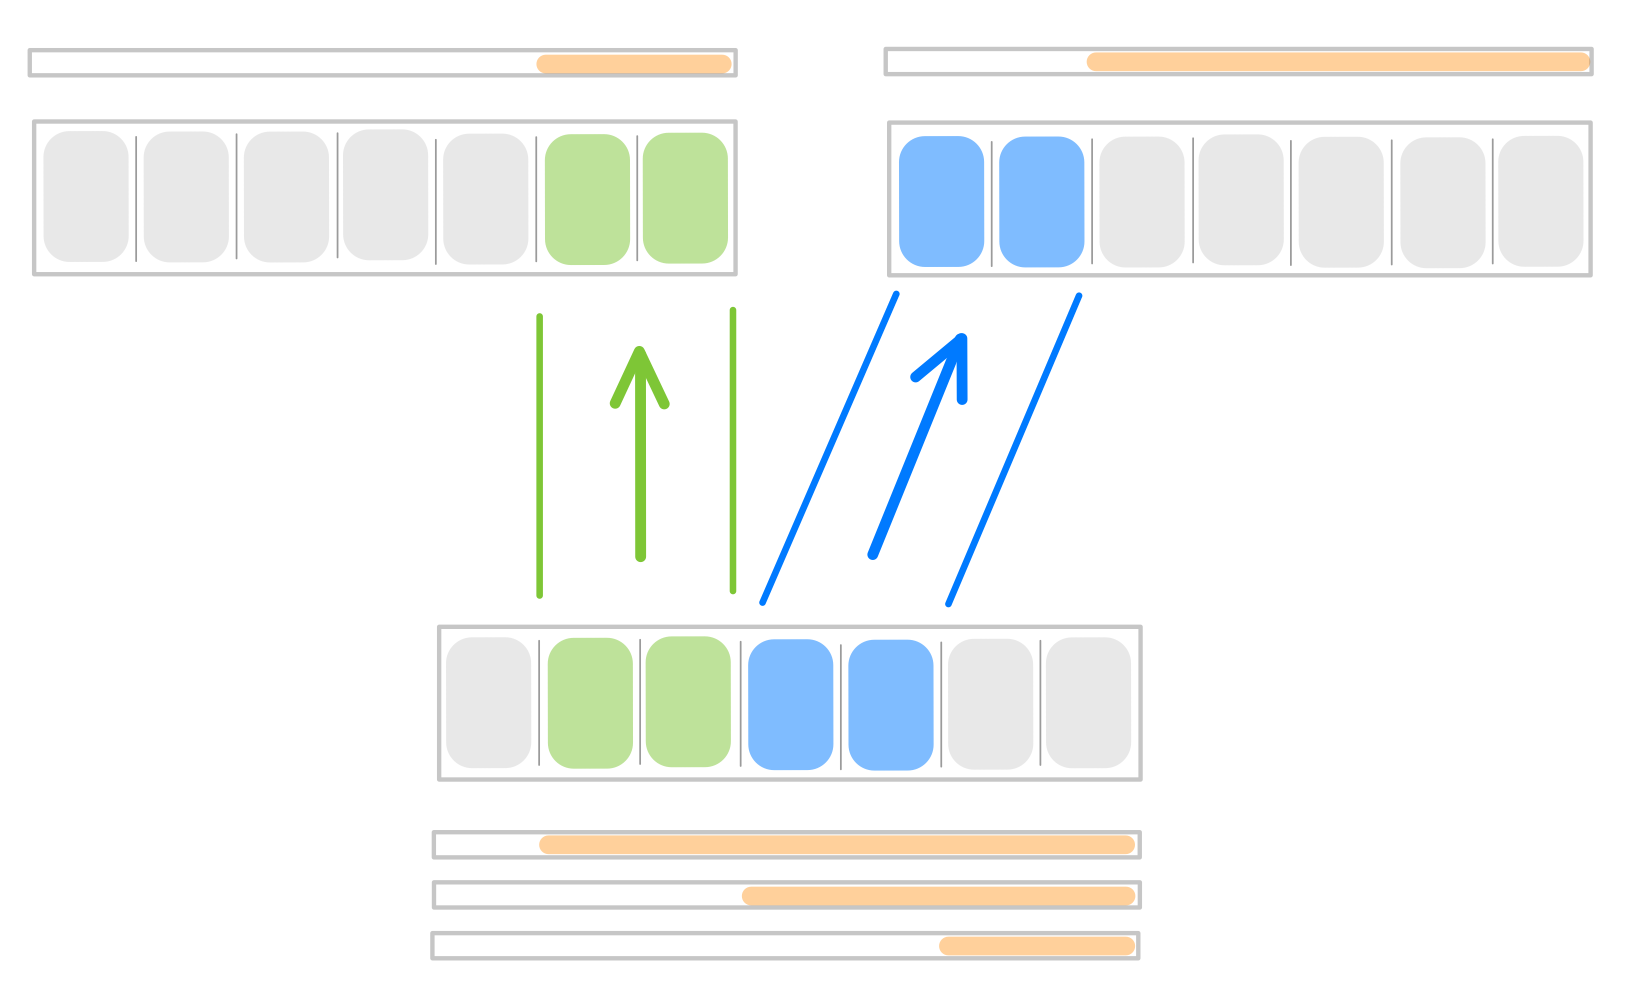
\includegraphics[width = 0.5\textwidth]{drawing/1_partial_to_2}
	\label{fig: one partial to two}
	\caption{Representation of the constraints implemented by $\onePartialToTwo$.}
\end{figure}
